159. \begin{figure}[ht!]
\center{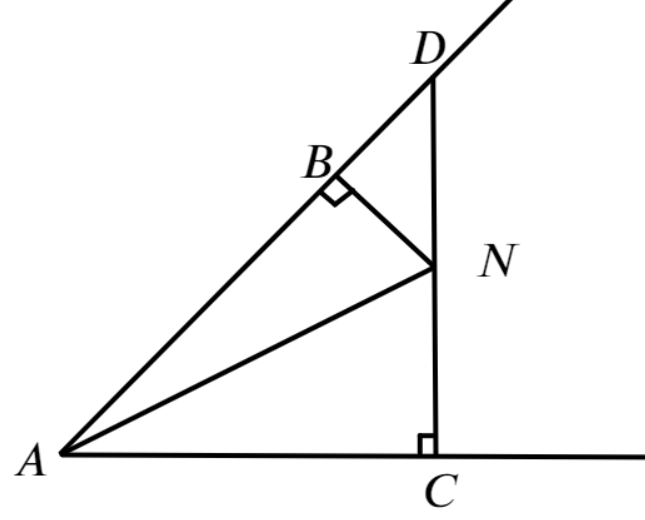
\includegraphics[scale=0.35]{g9-159.png}}
\end{figure}\\
Опустим перпендикуляры $NB$ и $NC$ ($NB=2$см, $NC=2\sqrt{2}$см) и продлим $NC$ до пересечения с $AB$ в точке $D.$ Найдём $\angle BDN=90^\circ-\angle A=45^\circ,$ значит треугольники $BDN$ и $CAD$ являются равнобедренными. Тогда $DN=\sqrt{BN^2+BD^2}=\sqrt{4+4}=2\sqrt{2}$см и $AC=CD=NC+DN=4\sqrt{2}$см. По теореме Пифагора для треугольника $ACN$ получим $AN=\sqrt{32+8}=2\sqrt{10}$см.\\
